\documentclass[10pt,a4paper]{article}

\usepackage[utf8]{inputenc}
\usepackage[T1]{fontenc}
\usepackage{amsmath,amssymb}
\usepackage{graphicx}
\usepackage{hyperref}
\usepackage{booktabs}
\usepackage{geometry}
\usepackage{parskip}
\usepackage[numbers]{natbib}
\usepackage{textcomp}
\usepackage{gensymb}
\usepackage{subcaption}
\usepackage{float}
\usepackage{listings}
\usepackage{tabularx}
\usepackage{array}

\setlength{\Urlmuskip}{0mu plus 1mu}

\lstset{
    basicstyle=\footnotesize\ttfamily,
    language=Python,
    keywordstyle=\bfseries,
    commentstyle=\itshape,
    breaklines=true,
    showstringspaces=false,
    numbers=none,
    frame=leftline,
    framesep=8pt,
    xleftmargin=1em,
    captionpos=b,
    aboveskip=1.2em,
    belowskip=0.6em
}

\DeclareCaptionFormat{custom}
{
    \small\textbf{#1#2}\textit{#3}
}
\captionsetup{format=custom}

\geometry{margin=4.5cm}

\hypersetup{
	unicode,
	hidelinks,
	pdfauthor={Giovanni Filippini},
	pdftitle={Assessing and Adapting CLIK-Diffusion for Tooth Alignment on Intraoral Scans},
    pdfsubject={Geometric evaluation and fine-tuning of CLIK-Diffusion on intraoral scans, including landmark coverage, simulated treatment targets, and sensitivity to diffusion noise.},
    pdfkeywords={Diffusion Models, Tooth Alignment, Intraoral Scans, Domain Transfer, Orthodontics},
	pdfproducer={Overleaf},
	pdfcreator={pdflatex}
}

\title{\textbf{Assessing and Adapting CLIK-Diffusion for Tooth Alignment on Intraoral Scans}}

\author{Giovanni Filippini$^1$\vspace{1.5mm} \\
{\small $^1$Università degli Studi di Milano} \\
    {\small \texttt{giovanni.filippini@studenti.unimi.it}}
}

\date{}

\begin{document}

\maketitle

\begin{abstract}
CLIK-Diffusion is a recent method for automatically aligning teeth. It detects anatomical landmarks on each tooth, moves them using a conditional diffusion model, and recovers the motion of each tooth. It was developed using cone-beam computed tomography. This report examines whether the published model is effective for intraoral scans, which are far more common in orthodontic practice, and the necessary modifications to make it useful for these scans. On 85 annotated Teeth3DS+ patients, the landmark detector places a landmark at a median distance of between 0.48 and 0.72\,mm from four of the six annotated classes; the other two can be computed from the crown's geometry. On 246 PrePostOrthodontic cases, whose targets are digitally simulated plans approved by orthodontists, the published model outperforms leaving the teeth where they are in 44\% of cases in rotation and 17\% in point-cloud distance. Retraining the diffusion stage alone increases these percentages to 70\% and 55\%, respectively. The retrained model also outperforms the average motion of each tooth in terms of rotation and translation, though not position. Of the clinical constraints implemented here, only the one on tooth orientation is helpful with these data. The diffusion network ignores its noisy input, so a single denoising step yields the same results as the original chain's two thousand steps. In practice, the model behaves like a deterministic regression network.
\end{abstract}


\section{Introduction}

Tooth repositioning is the orthodontic treatment used to establish a functional occlusion and an acceptable appearance, and it acts both on the alignment of the two arches and on the position of every individual tooth of the patient. Before starting any procedure the clinician has to define the arrangement those teeth should reach at the end of treatment. This is still done by hand on a digital model, moving and rotating one tooth at a time until the whole set satisfies a number of empirical criteria, such as the teeth of the two arches meeting correctly when the patient bites, every tooth having the right inclination and no rotation around its own axis, each tooth touching its neighbors without gaps, and the biting surfaces lying on an almost flat plane.\footnote{These criteria were codified by \citet{andrews1972} as the six keys to normal occlusion, from the study of 120 untreated dentitions with a naturally normal occlusion, and they are still widely used as the reference for what an ideal arrangement should look like.} Automatic tooth alignment aims to predict this target arrangement directly from the scans of the patient.

Formulated geometrically, the task is well posed. Given the dentition of a patient as a set of individual three-dimensional surfaces, an automatic method has to predict, for each tooth, the rigid transformation that maps it from its pretreatment pose to the pose it is expected to occupy once treatment is complete. TANet \citep{wei2020tanet} is one of the first learning-based methods for this task. It encodes the dentition with a point cloud network and regresses for every tooth the six parameters of a rigid motion, three for the rotation and three for the translation, a formulation kept by most of the later methods against which CLIK-Diffusion is compared.

CLIK-Diffusion \citep{DOU2025103746}, a Clinical Knowledge-informed diffusion model and the model studied in this report, departs from this formulation in two ways. Each tooth is described by a fixed set of anatomical landmarks placed on its surface instead of the six numbers of a pose, and the landmarks of the treated dentition are generated by a conditional diffusion model, from which the rigid motion of each tooth is then recovered in closed form. The landmark representation allows clinical rules to be written as differentiable penalties during training, which gives the method its name, and with it the authors report better results than all the earlier methods they compare against. CLIK-Diffusion was developed and trained on cone-beam computed tomography (CBCT), a volumetric X-ray modality that reconstructs the whole tooth, crown and root.\footnote{The crown is the portion of a tooth exposed above the gingival margin and the root is the portion anchored in bone. Only the former is accessible to an optical instrument.}

Intraoral scanning is a different acquisition modality, where an optical scanner records only the surfaces that are visible inside the mouth, so that every tooth is recovered as a hollow shell of its crown, but the acquisition takes a few minutes and involves no ionizing radiation. Scans of this kind are consequently acquired far more often in orthodontic practice than volumetric ones, and the public collections of treated cases that exist are built on them. Whether a model trained on tomographic reconstructions retains its accuracy when the input comes from an optical scanner is therefore a question with practical consequences, and it is the question this report addresses. It can be posed at all only because the released implementation includes a crown-only variant, which does not require root geometry.

Two public collections of intraoral scans support the work. The landmark stage is assessed on Teeth3DS+ \citep{ben2022teeth3ds}, whose manual annotations provide an independent reference for landmark locations. Alignment is assessed on the PrePostOrthodontic test split \citep{wang2024prepost}, which after conversion leaves 246 cases with a usable pretreatment model and corresponding digitally simulated post-treatment target. The second evaluation compares every prediction with a no-movement reference, which leaves each pretreatment dentition unchanged, and like every metric in this report it measures geometric agreement with the simulated target rather than clinical benefit.

\subsection{Objectives}

The project pursues three objectives, one for each step of the investigation. The first is to measure how closely CLIK's predicted landmarks cover the manual annotations of 3DTeethLand \citep{benhamadou2025teethland} on the annotated subset of Teeth3DS+, and how well the annotated classes can then be recovered one by one. The second is to evaluate the published model as-is on PrePostOrthodontic cases, comparing its predictions with the digitally simulated targets and determining which of its three stages accounts for the geometric error. The third is to fine-tune the generative stage on intraoral data and quantify what is gained by doing so, including which of the three clinical constraints still help on this data. Two further analyses grew out of these, one asking whether the diffusion network actually uses its noisy input and one asking whether a landmark with a given index marks the same anatomical position in different patients.


\section{Background}

\subsection{Denoising diffusion probabilistic models}
\label{sec:background-diffusion}

A denoising diffusion probabilistic model \citep{sohldickstein2015,ho2020ddpm} generates data by learning to invert a fixed corruption process. Given a clean sample $x_0$ and a noise schedule $\beta_t \in (0,1)$, with $\alpha_t = 1-\beta_t$, the forward process is a Markov chain that adds Gaussian noise over $T$ steps:
\begin{equation}
q(x_t \mid x_{t-1}) = \mathcal{N}\!\left(x_t;\, \sqrt{\alpha_t}\, x_{t-1},\, (1-\alpha_t)\mathbf{I}\right).
\end{equation}
Since a composition of Gaussian steps is again Gaussian, $x_t$ can be drawn directly from $x_0$ for any $t$ without traversing the chain, as $x_t = \sqrt{\gamma_t}\,x_0 + \sqrt{1-\gamma_t}\,\epsilon$ with $\gamma_t = \prod_{s \le t} \alpha_s$ and $\epsilon$ standard Gaussian noise, so training reduces to sampling a step index, corrupting the sample accordingly and asking a network to undo the corruption. Generation instead runs the learned reverse transition $p_\theta(x_{t-1} \mid x_t)$ from $t = T$ down to $t = 1$, each application taking as input the output of the previous one, and it is this recursion that turns a single-step denoiser into a sampler of the data distribution.

Two design choices of these models are important for this work. The first is what the network is trained to output. One possibility, the one chosen by \citeauthor{ho2020ddpm}, is the noise that was added at step $t$; the other is the clean sample $x_0$ itself. Either quantity can be computed from the other once $x_t$ and $t$ are known, because the forward process relates them by an invertible affine map, so the choice does not change what the model is able to represent. What it changes is the quantity that the loss rewards, and with it what is convenient to constrain. Predicting $x_0$ makes a reconstruction of the clean signal available at every step of the chain, which is what allows auxiliary losses to be written on the signal itself rather than on the residual noise, and that is why it was adopted for human motion synthesis by \citet{tevet2023mdm} and, for the same reason, by CLIK-Diffusion, whose clinical constraints are all expressed as functions of landmark coordinates. The second choice is the length of the chain, since sampling cost grows linearly in $T$ and a substantial body of work accelerates it either by using a non-Markovian forward process that allows a much shorter sampling chain \citep{song2021ddim} or by distilling the sampler into fewer evaluations. Both lines of work assume that the intermediate iterates carry information, that is, that the reverse transition really depends on its input, an assumption that this report tests for CLIK-Diffusion.

\subsection{CLIK-Diffusion}
\label{sec:clik}

CLIK-Diffusion replaces the pose regression of TANet with the generation of tooth landmarks, on the argument that a landmark set encodes position, orientation and shape at once and can therefore be constrained by explicit clinical rules, and it generates those landmarks with a conditional diffusion model. The method is built as three stages that run one after the other, a detector that turns every tooth into landmarks, a diffusion model that moves those landmarks to where the treatment should take them, and a closed-form fit that converts the displacement of the landmarks back into a rigid motion of the mesh.

\subsubsection{Landmark detection}

A fixed landmark set is defined per tooth type by expert dentists and comprises centroids, cusps, facial axis points and contact points, with eight landmarks on incisors and canines, nine on premolars and eleven on molars, so that a complete dentition of $N = 28$ teeth is described by exactly 256 landmarks. Four networks based on PointMLP \citep{ma2022pointmlp}, one per tooth type, take 2048 points sampled from the surface of a single tooth and emit one heatmap per landmark; heatmap regression is preferred to direct coordinate regression because it tolerates the ambiguity of manual annotation, and the coordinate is recovered as the argmax of the heatmap. The landmark count is fixed by construction rather than discovered, and dentitions with missing teeth are handled by zero padding the corresponding slots, so the representation always has 256 rows. The detected coordinates are concatenated with the landmark index and the tooth index to form the condition $L_c \in \mathbb{R}^{256\times5}$. A second input describes shape: for every landmark, 128 vertices are sampled inside a sphere of radius 2\,mm centered on it, whereas for the centroid the 128 vertices are drawn by farthest point sampling, which spreads them over the whole tooth instead of clustering them where the mesh is dense, so that the descriptor also carries a global view of the tooth.

\subsubsection{Conditional diffusion}

The generative stage is conditioned on both the condition $L_c$ and the shape descriptor produced by the detector. The denoising network that consumes them is a one-dimensional U-Net\footnote{A U-Net is an encoder-decoder network in which every decoder block also receives the output of the encoder block working at the same resolution, so that fine detail is not lost through the bottleneck. Here the convolutions run along the sequence of 256 landmarks rather than over an image, and the sequence keeps its length at every level, so that the levels differ only in their number of channels.} over the 256 landmark slots, whose input channels concatenate the current iterate, the condition and the descriptor, after a three-layer perceptron has reduced the descriptor to sixteen dimensions. All the quantities that govern the diffusion are the ones the authors report among their implementation details, namely a chain of $T = 2000$ steps with $\beta_t$ growing linearly from $10^{-6}$ to $10^{-2}$, and, as in the motion model of \citeauthor{tevet2023mdm}, the network predicts the clean target landmarks at every step, so that the reconstruction term is:
\begin{equation}
\mathcal{L}_{\text{Base}} := \mathbb{E}_{t\sim\mathrm{Uniform}\{1,\ldots,T\}}\left[\left\lVert L_{\text{target}} - \hat{L}_{\text{target}}(t)\right\rVert_2^2\right].
\label{eq:base}
\end{equation}
Clinical knowledge enters as three penalties on the predicted landmarks, ordered from the global to the local scale and combined into:
\begin{equation}
\mathcal{L}_{\text{Joint}} := \mathcal{L}_{\text{Base}} + \lambda_1 \mathcal{L}_{\text{Arch}} + \lambda_2 \mathcal{L}_{\text{Inter}} + \lambda_3 \mathcal{L}_{\text{Individual}},
\end{equation}
with $\lambda_1 = 0.1$, $\lambda_2 = 10^{-3}$ and $\lambda_3 = 10^{-2}$. The dental arch term projects the landmarks onto the horizontal plane of the canonical jaw frame, fits a fourth-order polynomial through the mean coordinate of each tooth and penalizes the squared difference between the five coefficients of the predicted curve and those of the target curve, a curve widely used in clinical practice to describe the shape of the dental arch. The inter-tooth term has two components, a contact loss over the thirteen pairs of adjacent teeth in each arch that draws the contact landmark of one tooth towards that of its neighbor, and a collision loss that penalizes query points which come to lie inside a neighboring tooth. The test is made on a signed distance field \citep{park2019deepsdf}, which gives for every point of space its distance to the surface of a tooth with a negative sign when the point lies inside it, precomputed once per tooth and carried along by the predicted rigid motion. The collision loss carries its own weight $\lambda_4 = 10^{-3}$ inside $\mathcal{L}_{\text{Inter}}$ and therefore enters the joint objective with an effective weight of $10^{-6}$. The individual-tooth term is one minus the cosine similarity between the predicted and the target root-crown and distal-mesial vectors, and thus constrains orientation while remaining indifferent to position. The root-crown vector is computed from the crown landmarks and the centroid alone, so it exists also for crowns without roots.

\subsubsection{Rigid transformation}

What the diffusion model predicts is a point cloud of displaced landmarks, which cannot directly relocate the teeth and must be converted into rigid transformations applied to the surface meshes. For each tooth the rigid motion that best carries its detected landmarks onto its predicted ones is recovered in closed form by the Kabsch algorithm \citep{kabsch1976}, which returns the rotation minimizing the squared distance between two sets of paired points, and applied to the tooth mesh, so the output is rigid by construction and whatever part of the predicted landmark cloud is not a rigid motion of the input is discarded.

\subsubsection{Training data and released variants}

Those three stages were fitted on 2224 CBCT scans acquired at a single hospital under uniform acquisition parameters, of which 1955 passed quality control. Of these, 1507 were used for the landmark detector and 448 paired pre and post treatment cases for the diffusion model, split into 348 for training and 100 for testing. The generative stage is therefore fitted on a few hundred dentitions, which bounds its capacity to generalize across broader populations. The group of patients behind those pairs is narrow as well, 448 Chinese patients treated in one hospital, aged between 11 and 48 years and female in 71.9\% of cases, which bounds what can reasonably be expected of the model outside that population. The released implementation offers two variants, one for complete teeth including roots and one for crowns alone;\footnote{\url{https://github.com/ShanghaiTech-IMPACT/CLIK-Diffusion}. The experiments reported here use a fork of that repository with device selection patched for Apple Silicon, included as a git submodule.} only the second is applicable to optical scans.

The two kinds of crown remain distinct objects even under that variant. A crown obtained from a tomography is segmented out of a voxel grid,\footnote{A voxel is the three-dimensional counterpart of a pixel, so a tomographic reconstruction is a regular lattice of density samples from which surfaces have to be extracted by segmentation.} whereas a crown obtained from an intraoral scan is measured directly by the scanner, so the two differ in resolution and in surface detail and are cut at the gingival margin in different ways. The authors explicitly acknowledge this gap, observing that optical data lacks root structures altogether while retaining structures that their own tomographic data lacks.

\subsection{Datasets}

Two datasets are used, one for the first objective and one for the remaining two.

Teeth3DS+ collects 1800 intraoral scans from 900 patients, with the upper and lower jaw acquired separately, and provides a per-vertex tooth segmentation labeled in the FDI two-digit notation.\footnote{Distributed at \url{https://crns-smartvision.github.io/teeth3ds}. FDI, standardized as ISO 3950 \citep{iso3950}, identifies a tooth by two digits, the first giving the quadrant of the mouth and the second the position of the tooth counted from the midline, so that 46 is the lower right first molar. The Universal notation instead numbers the teeth consecutively from 1 to 32. CLIK indexes teeth in the Universal notation, so the labels are renumbered during conversion.} The 3DTeethLand challenge adds manual landmark annotations on 340 of those scans, released as a training set of 240 and a test set of 100, and defines six classes, namely the mesial and distal points, the cusp, the inner and outer points on the tooth-gingiva junction, and the facial axis point at the center of the buccal surface.\footnote{Mesial and distal denote the side of a tooth facing the midline of the arch and the opposite side, buccal the side facing the cheek or lip and lingual the side facing the tongue. A cusp is a pointed elevation of the biting surface, and the third molars, or wisdom teeth, are the last teeth of each arch.} Eighty-five patients of the training set carry annotations on both arches and form the evaluation set used here. The value of this dataset here is that it supplies an independent, manually annotated reference for landmarks on optical scans, so the first stage of CLIK can be assessed without any post-treatment information being available.

PrePostOrthodontic provides 1060 pairs of pretreatment dental models and digitally simulated post-treatment targets from 435 patients treated at Beijing Stomatological Hospital. The targets are designed by technicians and approved by orthodontists; they are not follow-up scans recording clinical outcomes. Aligner treatment usually proceeds in phases, and every phase is a separate case that pairs the dental model at its beginning with the target designed for it, so one patient can contribute several cases. Each model is segmented into individual teeth, and corresponding tooth meshes are, with rare exceptions, rigidly repositioned copies, so the geometric transform from each pretreatment tooth to its target can be recovered directly. The official split contains 810 training and 250 test cases.\footnote{Deposited at \url{https://doi.org/10.5281/zenodo.11392406}. The 1060 pairs are what remains of the 1130 originally collected, once models of insufficient quality were filtered out.}

External validation on PrePostOrthodontic has also been reported by the authors of CLIK-Diffusion. Their results provide a benchmark on the same dataset. However, the comparison is not direct: for their evaluation, the authors retrained their landmark detector using dentist-annotated tooth models from the dataset. In contrast, the present evaluation uses the released detector without adaptation. Therefore, the published figures are contextual and should not be used to attribute performance differences solely to the diffusion model.


\subsection{Evaluation metrics}
\label{sec:metrics}

The four geometric metrics used in the original work are computed against the digitally simulated target. Three compare, tooth by tooth, the transformation predicted by the model with the transform from the pretreatment tooth to its corresponding target. The rotation error is the angle of the rotation separating the two, recovered from the trace of their product:
\begin{equation}
2\cos(\lvert\theta\rvert) = \operatorname{trace}\!\left(R_{gt}^{-1}R_{pred}\right) - 1,
\qquad \Delta_{\text{Rotation}} = \lvert\theta\rvert,
\end{equation}
and is expressed in degrees. The translation error $\Delta_{\text{Translation}}$ is one third of the $L_1$ distance between the predicted and target translation vectors, both expressed in the recentered frame of the dentition, in millimeters. The point-cloud error $\Delta_{\text{PointCloud}}$ compares corresponding points on the predicted tooth and its simulated target, using their mean Euclidean distance, also in millimeters.

The fourth metric does not involve the treated dentition at all and asks instead whether the predicted one is physically possible. Query points are sampled on each tooth and their signed distance to the neighboring teeth is evaluated, a negative value meaning that the point has ended up inside a neighbor, and the metric averages that distance over the penetrating points alone:
\begin{equation}
\Delta_{\text{Collision}} = \frac{\sum_{i=1}^{N}\sum_{j=1}^{M_i}\left\lvert\min\!\left(\mathrm{SDF}(q_{i,j}),\,0\right)\right\rvert}
{\sum_{i=1}^{N}\sum_{j=1}^{M_i}\mathbf{1}\!\left(\mathrm{SDF}(q_{i,j}) < 0\right)},
\end{equation}
where $N$ is the number of teeth and $M_i$ the number of query points on the $i$-th one. It therefore reports how deep the overlaps are, and it is reported here together with the fraction of points involved, which says how widespread they are.

The first three metrics are also computed for the identity transform applied to every tooth, which leaves the pretreatment dentition unchanged and is called the no-movement reference. A prediction with higher error than this reference is geometrically farther from the target than the dentition it started from, and for this reason the report gives, besides the medians, the fraction of test cases in which each prediction has lower error than the reference.

\section{Methods}

\subsection{Data conversion and the canonical jaw frame}

CLIK works on individual teeth rather than on a whole arch, so the first step is to split every arch into its teeth. The original files are never modified, since the conversion reads them and writes a separate copy in the format that CLIK expects. PrePostOrthodontic distributes each arch as a single mesh accompanied by a segmentation that lists the vertices belonging to every tooth, so the converter recovers the faces of a tooth by matching those vertices back onto the arch mesh. Teeth3DS+ instead labels every vertex directly, and there a face is assigned to a tooth when at least two of its three vertices carry that label, which behaves sensibly at the boundaries between adjacent teeth and between a tooth and the gingiva. In both cases the teeth are then renumbered from FDI to the Universal notation, which CLIK uses both to select the detector matching the tooth type and to place the tooth within the dentition, so that leaving the original labels in place would misclassify every tooth. The two arches are finally merged and the dentition is recentered.

The final conversion step estimates the canonical jaw frame, a necessary operation since CLIK-Diffusion is not invariant to input orientation. Its diffusion model learned the shape of the dental arch in a fixed frame, with the anterior direction along $-x$, the patient's right along $+y$ and the upper arch along $+z$, and nothing in the architecture removes that dependence.

PrePostOrthodontic is not consistently oriented. Of its 250 test cases, 248 carry enough anatomy for the frame to be estimated, and only 61 of them share the orientation of the first case of the collection, in which the upper arch lies below the lower one along the vertical axis, while the other 187 have it above. The consequence is that a single rotation estimated on that case and applied to the whole collection presents the majority of dentitions to the model upside down. That is not a cosmetic error: in an earlier version of the pipeline, the misoriented inputs produced a median rotation error of 13.25\degree{}, compared with 9.41\degree{} for the no-movement reference on the same cases. Thus, the preprocessing artifact made the method appear worse than the reference; an experiment run in that state could have reached the opposite conclusion.

The frame is consequently estimated for each case from the anatomy itself. Three directions are derived from the tooth centroids, the anterior direction $a$ as the incisors minus the molars, the vertical $u$ as the upper arch minus the lower arch and the patient's right $r$ as the right teeth minus the left. These are not orthogonal as they stand, so they are normalized by the Gram-Schmidt process. The vertical direction is processed first, so that it is the one surviving unchanged. Since a rotation between two orthonormal frames is the product of one by the transpose of the other, the matrix carrying the case onto the canonical frame follows directly:
\begin{equation}
R = T \begin{bmatrix} a & r & u \end{bmatrix}^{\top},
\qquad T = \begin{bmatrix} e_{\text{ant}} & e_{\text{right}} & e_{\text{up}} \end{bmatrix},
\end{equation}
where the columns of $T$ are CLIK's three canonical axes. The determinant of $R$ is then checked, and a case for which it is negative is discarded rather than corrected, because a negative determinant would mirror the dentition and silently exchange left and right, which is anatomically impossible and would not show up in any of the metrics. Crucially, the same rotation matrix $R$ is applied to both the initial ($S_{\text{pre}}$) and target ($S_{\text{post}}$) meshes of a case, preserving relative geometry and ensuring that per-tooth rigid transformations remain identical before and after conversion.

\subsection{Target construction}
\label{sec:targets}

For each case, the pretreatment tooth mesh and its corresponding digitally simulated target mesh have matching vertices under a rigid transformation. This can be verified by aligning the vertices with the Kabsch algorithm, the same closed-form fit used in CLIK's final stage: for 99\% of the teeth the resulting root mean square deviation is below $2\cdot10^{-4}$\,mm, which is numerical noise. The exceptions are 26 of the 6223 evaluated test teeth, which have the same number of vertices in the two meshes but a deviation between 0.1 and 7.7\,mm, and which are kept in the evaluation because removing them changes the median errors by at most 0.08\degree{} and 0.02\,mm and the share of cases beating the no-movement reference by at most one point. For all the other teeth the rigid transform from the pretreatment tooth to its target can therefore be recovered with negligible error.

Targets are consequently not produced by running the landmark detector a second time on the simulated target crowns. The detector is run once, on the pretreatment dentition, and the landmarks it produces are carried through the per-tooth transformation recovered from the meshes, so that writing $L^{(i)}$ for the landmarks detected on the $i$-th crown and $(R_i, t_i)$ for the rotation and translation that Kabsch returns for that same tooth, the target is simply the image of the detected landmarks under that motion:
\begin{equation}
L^{(i)}_{\text{target}} = R_i L^{(i)} + t_i .
\end{equation}
Two properties follow from this choice. The target corresponds one to one with the input, so the network is asked to move each landmark to its corresponding position in the simulated target. More importantly, the task remains well posed even where the detector places landmarks that are anatomically imprecise, because input and target are expressed in the same convention, imperfect or not, and what the network is asked to learn is the motion rather than the anatomy. As a check, on the test cases the centroid of the target landmarks of a tooth coincides with the centroid of the corresponding simulated post-treatment mesh to within 0.004\,mm in the worst case, confirming that the construction reproduces the target geometry.

A tooth is excluded from supervision in two circumstances, handled by clearing its entries in a validity mask defined over the 256 landmark slots. First, a tooth may be absent from the simulated target, leaving no target landmarks for that tooth. The available data do not establish whether this absence reflects a clinical extraction. Second, the pretreatment and simulated-target meshes may have different vertex counts, preventing the pointwise correspondence needed to recover the target transformation. The mask allows the reconstruction loss to ignore landmarks without a recoverable target and is stored alongside the tensors, so training never needs to consult the meshes again. Coordinates are stored in the normalized units used by the network, namely millimeters divided by 46, the scale constant of the released code.

\subsection{Pipeline architecture and portability}
\label{sec:pipeline}

The released implementation performs the three stages of the method in a single process, which is appropriate for inference but not for fine-tuning, where the generative stage has to be trained over the same landmarks for hundreds of epochs while the detection stage needs to produce them only once. The pipeline is therefore separated into four stages, of which stage A prepares the tensors described above, stage B trains the diffusion model, stage C samples the predicted landmarks and stage D recovers the rigid motions and writes the aligned dentition. Only stage B performs training, while stages A, C and D are used to evaluate any set of weights, published or fine-tuned. Stages A and D require the meshes, whereas stages B and C are pure tensor computation over the network and can be executed on any machine, which is what makes the expensive part of the work relocatable.

Separating the stages is only legitimate if the result is identical to what the original implementation produces, since otherwise a comparison between the published and the fine-tuned model would be between two different programs rather than between two sets of weights. This is not automatic, because the landmark detector is stochastic at inference time. The detector is built on PointMLP, which performs farthest point sampling internally at each of its encoder stages, and since that sampling starts from an index drawn at random the landmarks produced for a tooth depend on the state of the random number generator. Two consequences follow, both of which look like inefficiencies and are not. The detectors must be constructed after the seed is set, because instantiating a PointMLP consumes random numbers while initializing its weights, and seeding in the opposite order displaces landmarks by millimeters. The teeth must also be processed one at a time rather than as a batch, because the number of draws taken from the shared generator depends on how many teeth travel together, and batching a full dentition moves 161 of its 228 non-centroid landmarks onto a different vertex. Neither effect is a matter of numerical tolerance, and both were reproduced identically on the CPU and on the Metal backend, the interface through which Apple Silicon exposes its graphics processor. Throughput is recovered by processing several cases in parallel instead, which preserves the result because cases are independent and each process keeps its own faithful copy of the sequence of draws.

Portability follows from the same separation. The computing device is selected once at import time, a CUDA graphics card where one is present, otherwise the Metal backend of Apple Silicon and finally the CPU, with an environment variable to override the choice. On the machine used here, which has no CUDA device, every stage runs on Metal except stage D, which runs on the CPU because the rigid fit is solved in double precision and the Metal backend does not implement that data type, a restriction that costs nothing because the solve is cheap.

\subsection{Fine-tuning objective and clinical constraints}
\label{sec:objective}

Since the official training code is unavailable, the implemented loss terms were reconstructed from the equations in the paper. Every loss described here therefore follows the published equations, and small differences from the unreleased implementation of the authors cannot be excluded. The reconstruction term is the base loss of Equation~\eqref{eq:base}, restricted to the landmarks that actually have a target, which for a mask $m \in \{0,1\}^{256}$ over the landmark slots gives the masked mean:
\begin{equation}
\mathcal{L}^{m}_{\text{Base}} := \frac{\sum_{k=1}^{256} m_k \left\lVert L_{\text{target},k} - \hat{L}_{\text{target},k}(t)\right\rVert_2^2}{3\sum_{k=1}^{256} m_k},
\end{equation}
where the numerator sums the squared error over the valid landmarks only and the denominator counts their coordinates, three for each valid landmark, so that dividing by the number of valid landmarks makes the value independent of how many teeth are missing from a given case, and in a batch both sums run over all its cases together. The step index $t$ is drawn uniformly over the two thousand steps, independently for every case of a batch, as in the original formulation, and a variant was also implemented in which the noise level is drawn from a continuous range instead of from the discrete list of steps, as done by Palette \citep{saharia2022palette}, the image-to-image diffusion model from whose public reimplementation the released code of CLIK-Diffusion is derived.

The three clinical constraints were likewise reimplemented from the published equations, reusing the index tables shipped with the released code rather than redefining them. Those tables specify which landmarks belong to which tooth, which two of them are the contact points, which pairs of contact points face one another across adjacent teeth and which landmarks make up the crown, and using them is what keeps the reimplemented terms faithful to the original formulation. The collision term was deliberately left out, for two reasons. It requires a signed distance field precomputed and stored for every tooth, and it enters the joint objective with an effective weight of $10^{-6}$, which suggested, without this being tested, that it would have little influence on a fine-tuning of a few hundred epochs. Its absence is one of the limitations of this work.


\section{Experiments}

\subsection{Step 1: landmark quality on intraoral scans}
\label{sec:exp-step1}

The first experiment evaluates the landmark detector on its own, since every later stage of the method works on the landmarks it produces. The evaluation set consists of the 85 Teeth3DS+ patients whose two arches both carry annotations in the 3DTeethLand training set. Each scan is split into per-tooth meshes and processed by CLIK in crown-only mode using the official inference module distributed with the repository, launched as a separate process, so that the released code runs exactly as it does in the original repository. Only the landmarks are kept, because in Teeth3DS+ the upper and lower arches are not registered to each other and the alignment stages would therefore have nothing meaningful to predict.

For every annotated landmark the error is the distance to the nearest landmark produced by CLIK, whatever its type. This is a coverage measure rather than a class-by-class comparison, and the choice is deliberate, because the two landmark schemes were defined independently and comparing them class by class would measure a disagreement between two definitions rather than an error of the detector. A crown is a small object and any point on it lies only a few millimeters from any other, so a raw distance is hard to interpret, and the same measurement is therefore repeated with points drawn at random among the vertices of the same crowns. For every patient the two medians are combined into a skill score, defined as one minus the ratio between the distance obtained by CLIK and the one obtained at random, and the scores of the 85 patients are summarized by their median. The score is zero for a detector that does no better than chance, one for a perfect detector and negative for a detector that systematically misses the annotated region.

The metric is complemented by two simpler checks, the first of which verifies that the detector behaves normally on the new data, producing the expected number of landmarks for each tooth type, placing them on the surface and spreading them over the crown instead of collapsing them onto a single region, which is the typical failure of a network used outside its training distribution. The second is a completion experiment, which asks how well the six annotated classes can be recovered one by one. The outer point and the facial axis point, which CLIK does not cover, are computed directly from the crown geometry, the first as the most buccal vertex of the gingival margin and the second as the center of the buccal surface, while the landmarks of CLIK are relabeled into the other four classes with a mapping learned on a single annotated patient, by assigning each of its annotations to the nearest tooth and choosing, for every tooth type and class, the landmark of CLIK that lies closest to the annotations of that class. Each annotation is then compared only with completed landmarks of its own class, on the 84 patients not used to learn the mapping, and the skill score is computed in the same way against as many random points on the same crowns. The aim of this experiment is to understand which landmarks really need a learned detector and which ones follow directly from the geometry of the tooth.

\subsection{Step 2: CLIK as-is}

The published model was evaluated before retraining, so that its performance on the same cases could be compared with that of the fine-tuned model. The three stages of CLIK were run with the published weights on the 246 PrePostOrthodontic test cases for which both the pretreatment model and its simulated target could be converted. The predicted dentition was compared with the target. Inference was run one case at a time through the released script and took about forty seconds per case; the four metrics were computed for each tooth and aggregated per case, alongside the no-movement reference.

Some teeth cannot be scored, and since their exclusion is not random it is worth listing them. Of the 6700 teeth present in the pretreatment models, the 152 third molars are never predicted, because the scheme of CLIK covers only 28 teeth. A further 232 teeth are absent from the digitally simulated targets, 310 in all when the 78 absent third molars already counted above are included; the available data do not establish whether they were extracted during clinical treatment. The model nevertheless predicts a motion for them, moving their centroids by a median of 1.72\,mm. Finally, 93 teeth have different vertex counts between the pretreatment and simulated-target meshes, so the pointwise correspondence required to recover their target transforms and compute the point-cloud error is unavailable. The remaining 6223 teeth form the evaluation set.

Since the target motion of every tooth is known exactly, the same experiment can also be used to measure the error of each stage separately instead of only at the output, which was done on the first 40 test cases. For the landmark stage no manual annotation is needed, because the target crowns are the pretreatment crowns transformed into their simulated target poses, so the landmarks found on a target crown should coincide with those found on the pretreatment one once the target motion is applied, and any difference measures how repeatable the detector is under a change of pose. To know how small this difference can possibly be, the detector is also run twice on the same mesh with different random seeds, which gives the noise level caused by its own random sampling. For the diffusion stage the raw output of the network is recorded and the predicted landmarks are compared with the ideal ones, that is, with the detected landmarks moved by the target motion. For the rigid stage the error is the part of the predicted landmark cloud that is not a rigid motion of the input and is therefore discarded by the final fit.

The detected landmarks are also used to ask whether a landmark with a given index marks the same anatomical position in different patients, which matters because the diffusion model learns a displacement for every index. For each tooth position, the landmarks detected on the first 250 training cases are superimposed by Procrustes analysis, which removes translation, rotation and size, and are then brought back to the average size of that tooth, so that the spread of a landmark, its mean distance from its average position, is expressed in millimeters.

Both the random point sampling of the detector and the sampler of the diffusion model depend on the random seed, so a single run could in principle mistake an unlucky draw for a systematic error, and for this reason the whole evaluation was repeated with five seeds on 40 cases. The spread between seeds is then compared with the difference from the no-movement reference, whose significance is tested per case with a paired $t$-test and with the Wilcoxon signed-rank test.\footnote{The Wilcoxon signed-rank test compares two sets of paired measurements without assuming that their differences follow a normal distribution, as the $t$-test does. The original work uses a paired $t$-test. Here both tests are computed for the evaluation of CLIK as-is, where they agree, and Wilcoxon is used for all the other comparisons, consistently with the medians reported throughout.}

\subsection{Step 3: fine-tuning}
\label{sec:exp-step3}

The official splits are defined over cases. Of the 810 cases in the official training split, 803 could be converted and provided at least one usable tooth target; these were divided with a fixed seed into 703 training cases and 100 validation cases. Of the 250 official test cases, 246 passed the same processing steps and were reserved for final evaluation. Because a patient may contribute several treatment phases and the dataset does not distribute patient identifiers, cases of the same patient may fall on both sides of the split, and the paired tests, which treat every case as independent, should be read as case-level results. The split was therefore checked by comparing the crowns themselves, each summarized by its three principal extents and its area, which do not depend on its pose. This finds scans that were used in more than one case, but it cannot recognize two different scans of the same patient, because apart from identical scans the descriptors of different cases vary continuously and show no separate group of near matches.

Training starts from the published weights and uses the optimization settings reported by the authors, namely Adam, a gradient-based optimizer that adapts the step size of each parameter separately, with a learning rate of $5\cdot10^{-5}$ and batches of 48 cases. Keeping these values unchanged means that any difference in the results can be attributed to the data and to the loss rather than to the optimisation. The only setting that changes is the number of epochs, 300 instead of the 10000 of the original work, because here training starts from the published weights, so the network already knows the task and only has to adapt to a new modality. The number of epochs was chosen by looking at the validation loss, computed every five epochs on the reconstruction term alone, which becomes flat within the first ten to twenty epochs while the training loss keeps falling, as Figure~\ref{fig:training} shows. The 300 epochs are therefore a generous budget rather than a need, and the later epochs mostly fit the training cases more closely.

\begin{figure}[htbp]
\centering
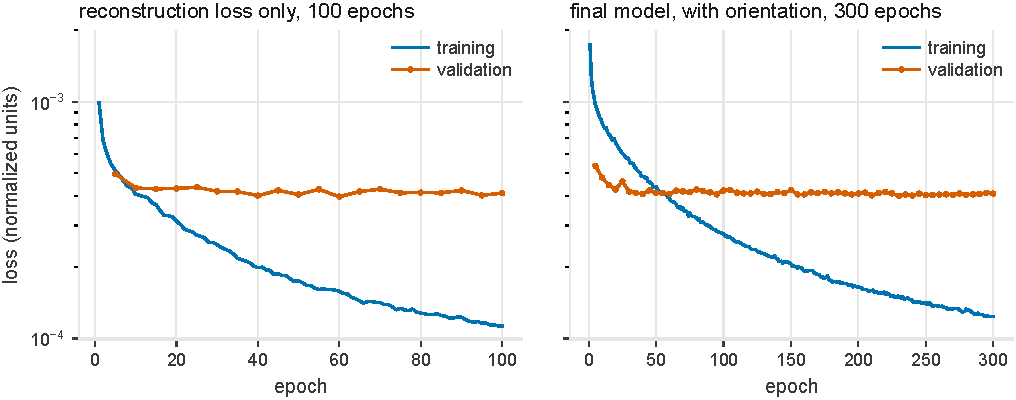
\includegraphics[width=\textwidth]{fig/training.pdf}
\caption{Training and validation loss of the run with the reconstruction loss alone, over 100 epochs, and of the final model, trained with the orientation term over 300 epochs. The validation loss is the masked reconstruction term in both panels, while the training loss of the final model also contains the orientation penalty, so its two curves are not directly comparable. In both runs the validation loss is flat after the first ten to twenty epochs while the training loss keeps falling.}
\label{fig:training}
\end{figure}

In a single training step, shown in Listing~\ref{lst:train}, the target dentition is corrupted with noise at a randomly drawn level, the network receives that level as input, as it does at inference, and predicts the clean landmarks directly, and the clinical terms are then computed on this prediction. This is what makes the clinical constraints usable during training, since they need a complete dentition to be evaluated on and a network that predicts the clean landmarks provides one at every step.

\begin{lstlisting}[float=htbp,caption={One training step of the generative pipeline, where \texttt{gamma} is the noise level of the sampled step, given by the cumulative product of the $\alpha_t$ up to it, \texttt{cond} the detected landmarks with their identifiers and \texttt{desc} the shape descriptor.},label={lst:train}]
cond, desc, target, mask = (x.to(device) for x in batch)
gamma = noise_level(net, cond.shape[0], device, continuous)
noise = torch.randn_like(target)
g     = gamma.view(-1, 1, 1)
noisy = g.sqrt() * target + (1.0 - g).sqrt() * noise

pred = net.denoise_fn(torch.cat([cond, noisy], dim=1), gamma, desc)

loss = masked_mse(pred, target, mask)
if weights:
    extra, parts = clinical_loss(pred, target, mask, weights)
    loss = loss + extra
\end{lstlisting}

The sampling procedure was also rewritten, so that the number of denoising steps could be chosen instead of being fixed. The sampler of CLIK always runs the whole schedule of two thousand steps, starting, as in the released code, from uniform rather than Gaussian noise, and the loop in Listing~\ref{lst:sample} reproduces it exactly but can stop after any number of steps. Stopping after two hundred steps means running the chain from step 1999 down to step 1800 and returning the clean dentition predicted there. On the laptop used for this work the full schedule takes 16.2 seconds per case, a little over an hour for the whole test set, while two hundred steps take 1.6 seconds, and the shorter setting was adopted only after the two had been compared on the whole test set with the same checkpoint.

\begin{lstlisting}[float=htbp,caption={The sampling loop modified to accept an arbitrary step count. \texttt{y\_0} denotes the predicted clean landmark set and \texttt{y\_t} the noisy iterate; setting \texttt{steps = 2000} reproduces the original sampling chain.},label={lst:sample}]
y_t = torch.rand_like(cond[:, :3])
y_0 = y_t
for i in reversed(range(net.num_timesteps - steps, net.num_timesteps)):
    t     = torch.full((b,), i, device=cond.device, dtype=torch.long)
    level = extract(net.gammas, t, x_shape=(1, 1))
    y_0   = net.denoise_fn(torch.cat([cond, y_t], dim=1), level, desc).clamp(-1, 1)
    mean, log_variance = net.q_posterior(y_0_hat=y_0, y_t=y_t, t=t)
    noise = torch.randn_like(y_t) if i > 0 else torch.zeros_like(y_t)
    y_t   = mean + noise * (0.5 * log_variance).exp()
return y_0
\end{lstlisting}

Separating the clean prediction from the noisy input in this loop also makes it possible to test whether the network uses the noisy input at all. For a fixed case and a fixed noise level, eight different noisy inputs are generated and given to the network while everything else is kept constant, and the spread of the eight predictions is compared with the spread of the eight inputs, averaged over the first eight test cases. At high noise levels a small ratio is expected even from a network that works as intended, because the input is then almost pure noise, whereas at low noise levels the input is almost the answer itself and a network that uses it should show a ratio close to one. The sensitivity measurement is evaluated across noise levels ranging from pure noise to a dentition that is almost at its target, both on the fine-tuned weights and on the published ones.

\subsection{Ablation of the clinical constraints}

Fine-tuning with a given loss shows how much the model improves overall, but not which terms of the loss are responsible for the improvement. Since the clinical constraints are the main contribution of CLIK-Diffusion, each of them is tested individually rather than by accumulating them as in the incremental study of the original work, because the question here is which individual constraints survive the change of acquisition modality. Every variant starts from the published weights and is trained for 100 epochs on the same 703 cases with the same optimizer, validation set and seed, so that two runs differ only in the constraint that was added, and the checkpoint retained is the one that minimizes the reconstruction term alone rather than the total loss, so that variants optimizing different objectives remain comparable. Five variants are trained in this way, namely the reconstruction loss alone, used as the reference, and the same loss with the dental arch term at its published weight of 0.1, with the contact term at $10^{-3}$, with the orientation term at $10^{-2}$, and with all three implemented terms together, a variant that tests whether the combined objective transfers but does not isolate the effect of any single term. All variants are evaluated on the first 100 test cases using the full sampling schedule, and each one is compared with the reference by a paired Wilcoxon test on the per-case errors. The comparison is paired because the differences between cases are much larger than those between variants, so an unpaired test would hide the effect of a constraint in the variability between cases.

A sixth variant was added after the first results, with the dental arch term at $10^{-3}$ instead of $10^{-1}$, in order to distinguish between a constraint that is unsuitable for this modality and one that simply has the wrong weight, since in the second case a smaller weight should turn its effect from negative to positive.

Two more variants were trained with the same protocol to check the training procedure itself rather than the constraints, both with the reconstruction loss and the orientation term. The first draws the noise level from a continuous range instead of the discrete list of steps, as Palette does, a change that should have little effect if the reconstructed training handles the noise correctly and that would improve the results if it did not. The second triples the number of epochs from 100 to 300 and is the run that produced the final model, whose retained checkpoint, chosen on the validation loss as for every run, comes from epoch 230. As a second reference besides the no-movement one, every test tooth is also moved by the average motion of its tooth position over the 703 training cases, computed as the mean rotation about the centroid of the tooth and the mean displacement of that centroid, so that a model can be compared with a prediction that ignores the patient altogether. A ninth run, the first to be made, used the reconstruction loss alone with the same split and settings and an earlier version of the training script; the reference of the ablation repeats it, so its results are not reported separately.

\subsection{Technology stack and cost}
\label{sec:stack}

All experiments run in a single conda environment with Python 3.12, in which \texttt{pytorch} provides the Metal backend, \texttt{trimesh} handles the meshes and the signed distance queries, \texttt{matplotlib} draws the charts, \texttt{pyvista} renders the three-dimensional views and \texttt{scipy} provides the statistical tests, and the exact version of each package is listed in a requirements file in the repository. The nine checkpoints released with CLIK, 3.6\,GB in total, of which the crown-only mode uses five, are not included in the repository and are downloaded from the link provided by the authors. The code of this project is available at \url{https://github.com/giovannifil-64/computer-vision}. Everything was run on a MacBook Pro with Apple Silicon and no CUDA device,\footnote{Configuration: Apple M5 chip with 10-core CPU (4 performance cores and 6 efficiency cores), 10-core GPU, and 24\,GB of Unified Memory.} using the Metal backend for every stage except the rigid fit. Claude Code, an AI coding assistant, was used for this project, particularly to have the code of the training stage written, which was not released by the authors and was rebuilt from the equations of the paper and their inference code.

Table~\ref{tab:stages} reports the cost of each stage of the pipeline. Overall, the nine training runs took 5.4 hours according to their logs, and sampling with the full schedule of two thousand steps, used for CLIK as-is, for the comparison of step counts and for the ablation, took about as long again.

\begin{table}[H]
\centering
\small
\begin{tabularx}{\textwidth}{@{}lXl@{}}
\toprule
Stage & Reads and writes & Cost \\
\midrule
A, prepare   & meshes $\rightarrow$ 0.3\,MB of tensors per case & 10\,s per case, 6\,s with four processes \\
B, train     & tensors $\rightarrow$ checkpoint        & 16\,s per epoch \\
C, predict   & tensors $\rightarrow$ landmarks         & 16.2\,s per case, 1.6\,s at 200 steps \\
D, transform & landmarks $\rightarrow$ meshes          & under a second per case \\
\bottomrule
\end{tabularx}
\caption{Input, output and computational cost of the four stages of the pipeline on the laptop used for this work.}
\label{tab:stages}
\end{table}


\section{Results}

\subsection{Validation of the split pipeline}
\label{sec:validation}

All the comparisons between CLIK as-is and the fine-tuned model rely on the assumption that the separated pipeline computes exactly what the original implementation computes, and this assumption was verified. Running three test cases through stages A, C and D and through the original single-process script gives the same dentitions up to numerical precision, with median differences per tooth of at most 0.0004\degree{} in rotation and 0.0001\,mm in translation and no tooth differing by more than 0.002\degree{} and 0.0005\,mm, far below any difference discussed in this report. Obtaining this agreement required reproducing the exact order in which the original code sets the random seed and builds the detectors, and processing the teeth one at a time instead of in batches, because getting either of these wrong moves the landmarks by millimeters while still producing plausible results. The first version of the pipeline, which set the seed in the wrong order, differed from the original by 9.5\% in rotation on 40 test cases, a difference large enough to be mistaken for a result.

\subsection{Step 1: landmark quality}

\begin{table}[htbp]
\centering
\small
\begin{tabularx}{\textwidth}{@{}Xrr@{}}
\toprule
Annotated class & Distance & Skill score \\
\midrule
Inner point       & 0.72\,mm & $+0.68$ \\
Mesial point      & 0.48\,mm & $+0.67$ \\
Cusp              & 0.55\,mm & $+0.66$ \\
Distal point      & 0.52\,mm & $+0.66$ \\
Outer point       & 2.53\,mm & $-0.05$ \\
Facial axis point & 2.94\,mm & $-0.54$ \\
\midrule
Overall           & 0.70\,mm & $+0.61$ \\
\bottomrule
\end{tabularx}
\caption{Median distance from each annotated landmark to the nearest landmark produced by CLIK, over the 85 Teeth3DS+ patients annotated on both arches in the 3DTeethLand training set. The skill score is computed for each patient as one minus the ratio between the median distance and the one obtained with random points on the same crowns, and the table gives its median over the patients; it is zero at chance level, one for a perfect detector and negative below chance.}
\label{tab:step1}
\end{table}

Table~\ref{tab:step1} shows that under the nearest-neighbour metric, the mesial, distal, cusp and inner-point annotations lie 0.48--0.72\,mm from the closest CLIK landmark (skill scores 0.66--0.68). Because matching ignores the predicted landmark's type, these distances indicate spatial coverage rather than class-specific semantic correspondence. For the mesial and distal points and the cusp the skill score is also stable across the 85 patients, with a standard deviation between 0.06 and 0.09, while for the inner point it varies more, with a standard deviation of 0.16, which is reasonable for a landmark defined on the border between tooth and gingiva. The outer point and the facial axis point, on the other hand, lie between two and a half and three millimeters away, with skill scores at or below chance. This does not mean that the detector fails on them, but that the landmark scheme of CLIK has nothing in those positions, since it defines its own facial axis point, which does not coincide with the one annotated in 3DTeethLand, and has no equivalent of the outer point. This result is consistent with a difference between the two landmark conventions, but the class-agnostic nearest-neighbour metric cannot determine how much of the distance is due to that mismatch rather than to detector localization.

The additional checks confirm this reading, since the detector produces the expected number of landmarks for each tooth type, places them on the surface and spreads them over the crown, so it does not behave like a network facing data it cannot handle. The completion experiment, measured class by class on the 84 patients not used for the mapping, shows that the two classes CLIK does not cover follow from the geometry of the crown, since the facial axis point lies at a median of 0.85\,mm from its annotation and the outer point at 1.60\,mm, with skill scores of 0.80 and 0.72. The relabeled landmarks of CLIK are less dependable. The cusp and the distal point stay at about 0.55 and 1.2\,mm whatever patient the mapping is learned on, but the mesial and inner points range from about 1 to 2.8\,mm depending on that choice, so a mapping learned on a single patient does not give a reliable class-by-class correspondence. Figure~\ref{fig:step1} shows the three sets of landmarks on the patient with the median skill score.

\begin{figure}[htbp]
\centering
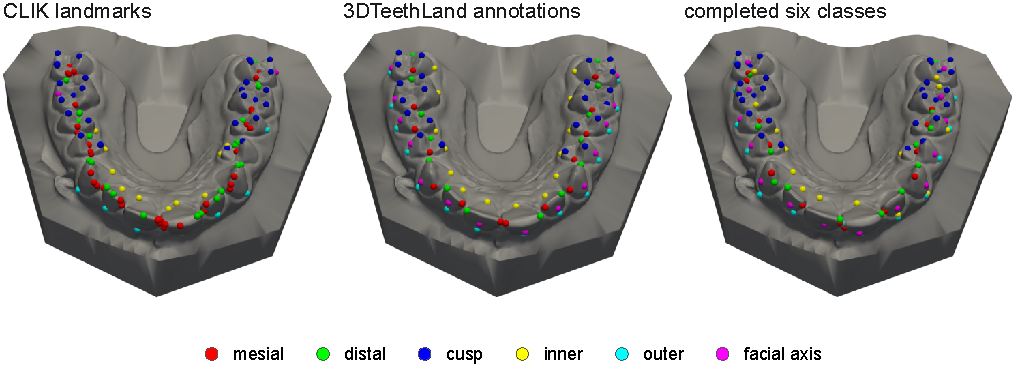
\includegraphics[width=\textwidth]{fig/step1_example.pdf}
\caption{Upper arch of the patient with the median overall skill score, with the landmarks detected by CLIK, the 3DTeethLand annotations and the six classes completed as in the completion experiment. The colors give the class of each annotation, and the landmarks of CLIK, which carry no class of their own, take the color of the nearest annotation.}
\label{fig:step1}
\end{figure}

\subsection{Step 2: CLIK as-is}
\label{sec:res-step2}

Table~\ref{tab:step2} reports the results of CLIK as-is as mean and standard deviation, the form used in the original paper, computed here over all teeth. The paper does not state whether its standard deviations are taken over teeth or over cases, so those of the last column may not be comparable with the others. The mean rotation errors are nearly identical, at 11.00\degree{} for CLIK and 11.05\degree{} for the no-movement reference. At the level of cases, however, CLIK has a higher rotation error than the reference in 56\% of them, and the paired Wilcoxon test on the per-case errors gives $p=0.02$, so the difference, although small, goes against CLIK. The last column reports the figures published by the authors on the same dataset only as a reference, since they were obtained after retraining the landmark detector on this dataset, which is exactly the adaptation that this experiment leaves out.

\begin{table}[H]
\centering
\small
\begin{tabularx}{\textwidth}{@{}Xrrr@{}}
\toprule
Metric & CLIK as-is & No movement & Paper \\
\midrule
Rotation error (\degree{})  & $11.00 \pm 8.56$ & $11.05 \pm 10.27$ & $6.69 \pm 2.56$ \\
Translation error           & $2.18 \pm 1.56$  & $2.01 \pm 1.79$   & $1.20 \pm 0.44$ \\
Point-cloud error           & $3.10 \pm 2.18$  & $2.15 \pm 2.06$   & $1.30 \pm 0.68$ \\
\bottomrule
\end{tabularx}
\caption{CLIK as-is on the PrePostOrthodontic test set, as mean and standard deviation over 6223 teeth of 246 cases, compared with the no-movement reference. The last column reports the figures published by the authors, obtained with a landmark detector retrained on this dataset. Rotation errors are reported in degrees; translation and point-cloud errors in millimeters.}
\label{tab:step2}
\end{table}

The prediction has lower error than the no-movement reference for 48\% of teeth in rotation, 43\% in translation and 24\% in point-cloud distance. Paired Wilcoxon tests on per-case median errors find a statistically significant difference from the reference for all three metrics, with $p$ values of $2\cdot10^{-2}$, $1\cdot10^{-8}$ and $4\cdot10^{-32}$, respectively. At the case level, Figure~\ref{fig:step2} shows that the prediction has greater rotation error than the no-movement reference in 56\% of cases and greater point-cloud error in 83\%.

\begin{figure}[H]
\centering
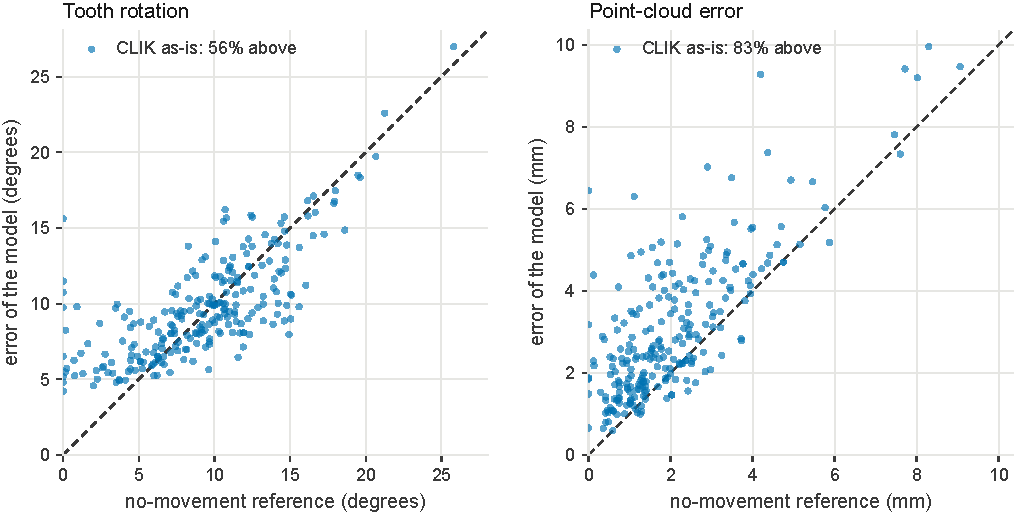
\includegraphics[width=\textwidth]{fig/clik_vs_baseline.pdf}
\caption{Each point represents one of the 246 test cases, for CLIK as-is with the published weights and two thousand denoising steps. The two panels compare the median rotation and point-cloud errors of the model with those of the no-movement reference, on the same axes as the corresponding figure for the fine-tuned model. Points above the diagonal are cases in which CLIK as-is has greater error than the reference, and the legend gives their share.}
\label{fig:step2}
\end{figure}

The median error by tooth type helps to localize the geometric error. For anterior teeth (incisors and canines), rotation errors are close to the no-movement reference (10.81\degree{} vs. 10.97\degree{} and 10.06\degree{} vs. 11.16\degree{}, respectively). Errors exceed the reference for premolars (9.19\degree{} vs. 8.91\degree{}) and particularly for molars (6.91\degree{} vs. 5.41\degree{}). Although molars have the lowest absolute rotation error, their error is still greater than the no-movement reference, indicating poorer agreement with the simulated target than leaving them unchanged.

Since the target transformation of every tooth is known exactly, the error can also be assigned to the single stages of the method, as reported in Table~\ref{tab:decomposition} for the first 40 test cases. Under a change of pose the landmark stage gives the same landmarks within a median of 0.10\,mm, a value partly degenerate, because in 19 of the 40 cases the two crowns are sampled with the same random draws and the landmarks coincide exactly. In the other cases the difference is of the order of the 0.31\,mm caused by the random sampling of the detector itself, so the detector is stable under a change of pose up to its own randomness. The rigid fit discards 0.71\,mm of non-rigid residual, a small amount showing that the predicted landmarks are almost a rigid motion of the input. The diffusion stage, instead, places the target landmarks 2.92\,mm away from the ideal ones, which accounts for almost all of the error, and this value is consistent with the median point-cloud error of 2.89\,mm measured on the meshes over all the teeth of the same cases, although the two are computed in different ways. Since the targets are built from the detected landmarks themselves, this decomposition measures how repeatable the detector is and how well the diffusion model reproduces motions expressed in those landmarks, not whether the landmarks are anatomically right, and an error in their meaning would appear as an error of the diffusion stage. The practical conclusion is that the error appears in the diffusion stage, which can be retrained on these targets without any new annotation, and this is why the fine-tuning of this work is applied there and not to the detector.

\begin{table}[H]
\centering
\small
\begin{tabularx}{\textwidth}{@{}lXr@{}}
\toprule
Stage & Measurement & Median \\
\midrule
Landmark detection & landmarks on the target crown against those on the pretreatment crown moved by the target motion & 0.10\,mm \\
Diffusion & predicted target landmarks against the detected ones moved by the target motion & 2.92\,mm \\
Rigid fit & the part of the predicted landmarks that is not a rigid motion of the input & 0.71\,mm \\
\bottomrule
\end{tabularx}
\caption{Error of each stage of CLIK as-is on the first 40 test cases, measured separately thanks to the exact target transforms. The 0.10\,mm of the landmark stage mixes 19 cases where the landmarks coincide exactly with cases at the 0.31\,mm noise level of the random point sampling inside the detector, and most of the error appears in the diffusion stage.}
\label{tab:decomposition}
\end{table}

Finally, the repetition with five seeds on 40 cases gives a spread between seeds of 0.075\,mm for the point cloud and 0.69\degree{} for rotation, against a median gap of 1.147\,mm between the point-cloud error of the model and that of the no-movement reference, about fifteen times larger. Given the insensitivity of the diffusion network to its noisy input, this spread comes mainly from the random sampling of the detector. It is small against the gap in point-cloud error, which is therefore systematic, and a single seed is sufficient for that metric, but in rotation it is comparable with the difference between CLIK as-is and the reference, so the conclusion that CLIK as-is is worse than leaving the teeth in place is weak for rotation.

\subsection{Landmark consistency}

Two properties of the detector have been measured so far, its stability under a change of pose and its coverage of the annotated landmarks. Neither of them, however, answers a third question that matters for the diffusion model, namely whether a landmark with a given index corresponds to the same anatomical position in different patients. The diffusion model learns a displacement for every landmark index, and this is only possible if every index has a stable meaning across the population.

\begin{figure}[H]
\centering
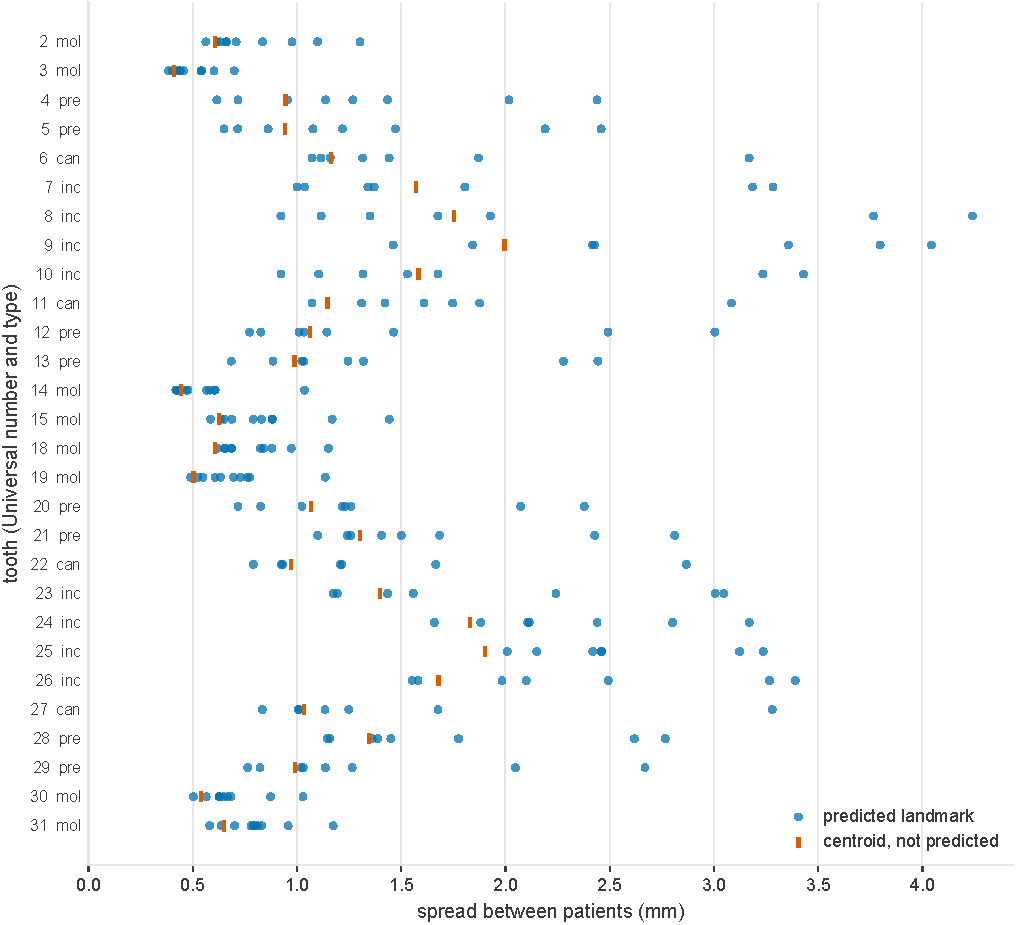
\includegraphics[width=\textwidth]{fig/landmark_spread.pdf}
\caption{Spread of each landmark between patients, one row per tooth position, on the first 250 training cases, with between 202 and 243 teeth per position, measured as the mean distance of the landmark from its average position after Procrustes superimposition. The centroid is computed from the mesh and not predicted by the network, so it shows how much the crown itself varies.}
\label{fig:spread}
\end{figure}

Figure~\ref{fig:spread} answers this question for every tooth position. The centroid is shown as a reference, since it is computed from the mesh rather than predicted, but it is not a lower bound, because a landmark placed on a sharp feature can be more stable than the center of the crown. With this reading, 31 of the 228 non-centroid landmarks vary more than twice as much as their centroid, thirteen of them on the premolars. In absolute terms, however, the least stable landmarks are those of the anterior teeth, whose spread reaches 3.0 to 4.2\,mm on the incisors and 2.9 to 3.3\,mm on the canines, against at most 0.7 to 1.4\,mm on the molars.

This is an unfavorable situation, because the anterior teeth are also the ones that treatment moves the most, so the least stable landmarks are found where the model most needs to be accurate. It is at least in part a property of the representation, since the shape of the anterior crowns varies considerably between individuals, and it limits what can be obtained by fine-tuning a model built on this representation.

\subsection{Ablation of the clinical constraints}

\begin{table}[H]
\centering
\small
\begin{tabularx}{\textwidth}{@{}lrrr>{\raggedright\arraybackslash}X@{}}
\toprule
Constraint (weight) & Rotation & Point cloud & Improved & Outcome \\
\midrule
Base loss only                       & 8.04\degree{}           & 1.62\,mm & --      & reference \\
$+$ dental arch (0.1)                & 15.04\degree{}          & 2.93\,mm & 0/100   & harmful, $p = 4\cdot10^{-18}$ \\
$+$ dental arch (0.001)              & 9.77\degree{}           & 1.73\,mm & 11/100  & still harmful, $p = 4\cdot10^{-16}$ \\
$+$ inter-tooth contact ($10^{-3}$)  & 7.93\degree{}           & 1.61\,mm & 53/100  & no measurable effect, $p = 0.52$ \\
$+$ tooth orientation ($10^{-2}$)    & \textbf{7.38\degree{}}  & 1.59\,mm & 66/100  & helps, $p = 4\cdot10^{-4}$ \\
Combined terms$^{\ast}$              & 12.68\degree{}          & 2.86\,mm & 0/100   & harmful, $p=4\cdot10^{-18}$ \\
\bottomrule
\end{tabularx}
\caption{Each clinical constraint against the reconstruction loss alone, over the first 100 test cases, with the median rotation and point-cloud errors, the number of cases on which the variant improves on the base loss in rotation and the paired Wilcoxon $p$ value. On these cases the no-movement reference is 8.95\degree{} and 1.52\,mm. The combined variant includes the arch, contact and orientation terms; the collision loss was omitted.}
\label{tab:ablation}
\end{table}

Table~\ref{tab:ablation} shows that only one of the three constraints helps when the model is fine-tuned on these data. The orientation term reduces the median rotation error from 8.04\degree{} to 7.38\degree{} and improves 66 cases out of 100, a difference that is significant with $p = 4\cdot10^{-4}$. The contact term has no measurable effect, since it changes the median by about a tenth of a degree and improves 53 cases while worsening 47, which is what a term without any effect would produce, and it is also small, between 1.5 and 13\% of the reconstruction loss from the first to the last epoch. The arch term, finally, is clearly harmful, as it almost doubles the rotation error and does not improve a single case out of a hundred.

The sixth variant helps to interpret this last result, since reducing the weight of the arch term by a factor of a hundred reduces the damage, from 15.04\degree{} to 9.77\degree{}, but does not make the effect positive, with only eleven cases out of a hundred improving and a result that is still significantly worse than the reconstruction loss alone. This does not settle whether the constraint is unsuited to this data or simply too heavy, however, because in the normalized units used here the term is very large. During the first epoch the weighted arch term is about two thousand times the reconstruction loss at the published weight and still about thirty times at the reduced one, and at the end of the reduced run the two are of the same size, so even the smaller weight never makes the arch term a minor part of the objective.

Combining the three implemented constraints, namely arch, contact and orientation, gives a rotation error of 12.68\degree{}, worse than both the reconstruction loss alone and the no-movement reference. In this ablation, the arch term dominates and the orientation term does not compensate for it. The implemented constraints therefore do not all help on these data. The experiment cannot tell, however, how much of this comes from the change of modality and how much from the reimplementation, since the loss terms had to be rebuilt without the original code and nothing here tests them on tomographic data. On these 100 cases no variant reaches the no-movement reference in position, where the best one, with the orientation term, has a median point-cloud error of 1.59\,mm against 1.52\,mm.

\subsection{Step 3: fine-tuning}
\label{sec:res-step3}

Table~\ref{tab:step3} compares CLIK as-is with the fine-tuned model, trained for 300 epochs with the reconstruction loss and the orientation term, the only constraint that helps in the ablation, on the 246 test cases. The two model columns share the same landmark detection and the same evaluation code, so the only difference between them is the set of weights of the diffusion model. The upper part of the table shows that fine-tuning the diffusion stage alone brings all three median errors below the no-movement reference, with rotation going from 9.28\degree{} to 7.38\degree{} against a reference of 9.49\degree{}, a value that coincides by chance with that of the orientation variant of the ablation, trained for 100 epochs and evaluated on the first 100 cases, translation from 1.84 to 1.32 against 1.76, and point-cloud error from 2.56\,mm to 1.58\,mm against 1.72\,mm. Every one of these changes is significant, with $p < 10^{-32}$ for the paired Wilcoxon test. In the form used by the original paper, as mean and standard deviation over the 6223 teeth, the fine-tuned model reaches $8.85 \pm 7.57\degree{}$, $1.62 \pm 1.31$ and $1.94 \pm 1.56$\,mm, against the $6.69 \pm 2.56\degree{}$, $1.20 \pm 0.44$ and $1.30 \pm 0.68$\,mm that the authors report after retraining the detector.

\begin{table}[H]
\centering
\small
\begin{tabularx}{\textwidth}{@{}Xrrrr@{}}
\toprule
 & CLIK as-is & CLIK fine-tuned & No movement & Mean motion \\
\midrule
\multicolumn{5}{@{}l}{\textit{Median error per case}} \\
Rotation error (\degree{}) & 9.28 & \textbf{7.38} & 9.49 & 8.58 \\
Translation error          & 1.84 & \textbf{1.32} & 1.76 & 1.68 \\
Point-cloud error          & 2.56 & \textbf{1.58} & 1.72 & 1.65 \\
\midrule
\multicolumn{5}{@{}l}{\textit{Cases on which the model beats no movement}} \\
Rotation error     & 44\% & \textbf{70\%} & -- & 64\% \\
Translation error  & 33\% & \textbf{69\%} & -- & 54\% \\
Point-cloud error  & 17\% & \textbf{55\%} & -- & 63\% \\
\bottomrule
\end{tabularx}
\caption{CLIK as-is and fine-tuned on the 246 test cases, together with the no-movement reference and the mean-motion reference, which moves every tooth by the average motion of its position in the training cases. The upper part reports median errors per case; the lower part gives the percentage of cases in which each model has lower error than the no-movement reference. Both models use the same landmark detection and therefore differ only in the diffusion-model weights. Rotation errors are reported in degrees; translation and point-cloud errors in millimeters.}
\label{tab:step3}
\end{table}

The lower part of the table reports the share of cases in which a model has lower geometric error than the no-movement reference. For CLIK as-is, this holds in 44\%, 33\%, and 17\% of cases for rotation, translation, and point-cloud distance, respectively. After fine-tuning, these proportions rise to 70\%, 69\%, and 55\%. Fine-tuning therefore improves geometric agreement with the simulated target in more cases, although the point-cloud error is lower than the reference in only 55\% of cases. Tested directly against the reference, the fine-tuned model is better with $p < 10^{-12}$ in rotation and in translation, while for the point-cloud error the paired Wilcoxon test gives $p = 0.02$ and a sign test on the 135 cases out of 246 gives $p = 0.14$, so the advantage in position is small. For CLIK as-is the median rotation error per case is slightly below the reference, 9.28\degree{} against 9.49\degree{}, while the model is worse on 56\% of the cases, because the two medians summarize the two distributions separately whereas the share of cases compares them case by case. Figure~\ref{fig:step3} shows the case-level errors of the fine-tuned model, to be read against those of CLIK as-is in Figure~\ref{fig:step2}.

The mean-motion reference is a harder test. Moving every tooth by the average motion of its position already improves on leaving the teeth in place, with lower error than the no-movement reference in 64\%, 54\% and 63\% of the cases. The fine-tuned model is clearly better than this average in rotation and in translation, on 72\% of the cases with $p < 10^{-15}$ in both, but not in position, where it is better on 55\% of the cases and the paired Wilcoxon test gives $p = 0.28$. In position, therefore, the fine-tuned model does not yet do better than a prediction that ignores the patient.

The check on the split finds four test cases whose pretreatment crowns are, for most teeth, the same scans as those of a training case, and one of them duplicates a training case completely, targets included. Removing these four cases changes the medians of the fine-tuned model by at most 0.01 and its shares of cases by at most one point, so the reused scans do not affect the results, while different scans of the same patient remain possible and cannot be detected in this way.

\begin{figure}[H]
\centering
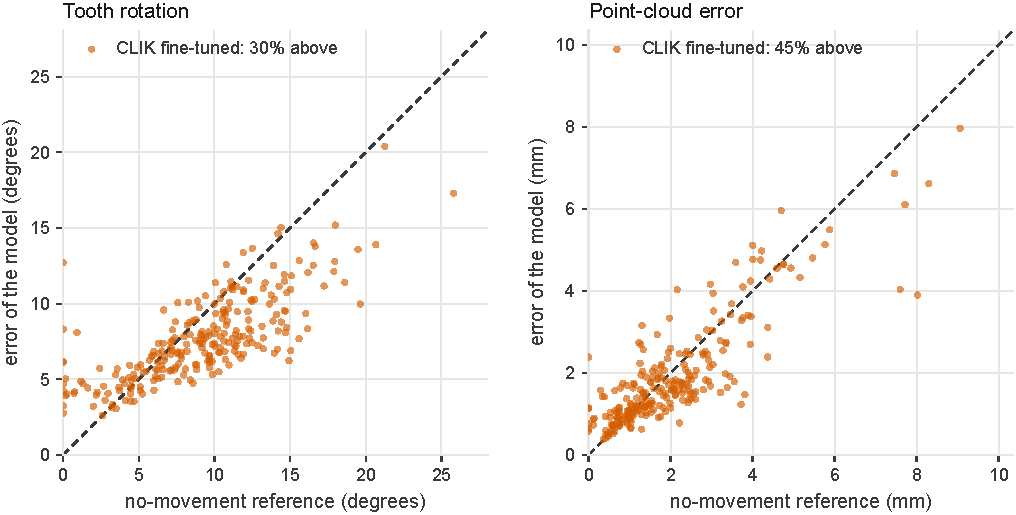
\includegraphics[width=\textwidth]{fig/tuned_vs_baseline.pdf}
\caption{Each point represents one of the 246 test cases, for the final fine-tuned model, trained for 300 epochs and sampled with two hundred denoising steps. The two panels compare the median rotation and point-cloud errors of the model with those of the no-movement reference, on the same axes as the corresponding figure for CLIK as-is. Points above the diagonal are cases in which the model has greater error than the reference, and the legend gives their share.}
\label{fig:step3}
\end{figure}

The two model columns of the table were sampled differently, CLIK as-is with the full schedule of two thousand steps and the fine-tuned model with two hundred steps. This does not affect the comparison, because the two settings were compared on the same checkpoint, a model trained for 100 epochs with the same loss, and gave 7.40\degree{}, 1.36 and 1.57\,mm with two thousand steps against 7.40\degree{}, 1.36 and 1.58\,mm with two hundred. The relative changes of $+0.03\%$, $-0.04\%$ and $+0.4\%$ are about a hundred times smaller than the differences between the two models, the cases are split roughly evenly between improvements and deteriorations, and the paired Wilcoxon test gives $p$ values of 0.52, 0.22 and 0.80. On the final model two thousand steps give 7.35\degree{}, 1.33 and 1.57\,mm, within 0.34\% of the values in the table, and shares of cases within one point of them, although the point-cloud difference of 0.19\% is significant ($p = 2\cdot10^{-5}$).

The fine-tuned model also underestimates the size of the motion, as Figure~\ref{fig:calibration} shows. Over the 6223 teeth of the test set, the median predicted translation is 0.86 times the median target translation and the median predicted rotation 0.64 times the median target rotation, while the correlations between predicted and target motion are 0.54 for translation and 0.56 for rotation, so the predictions point in the right direction but stop short of the target, especially in rotation. CLIK as-is behaves differently, since it moves the teeth by 1.31 times the target translation and 0.77 times the target rotation with correlations of only 0.13 and 0.34, so fine-tuning mostly makes the predictions follow the target and brings the translation below its size, while the rotation was already short of it.


\begin{figure}[H]
\centering
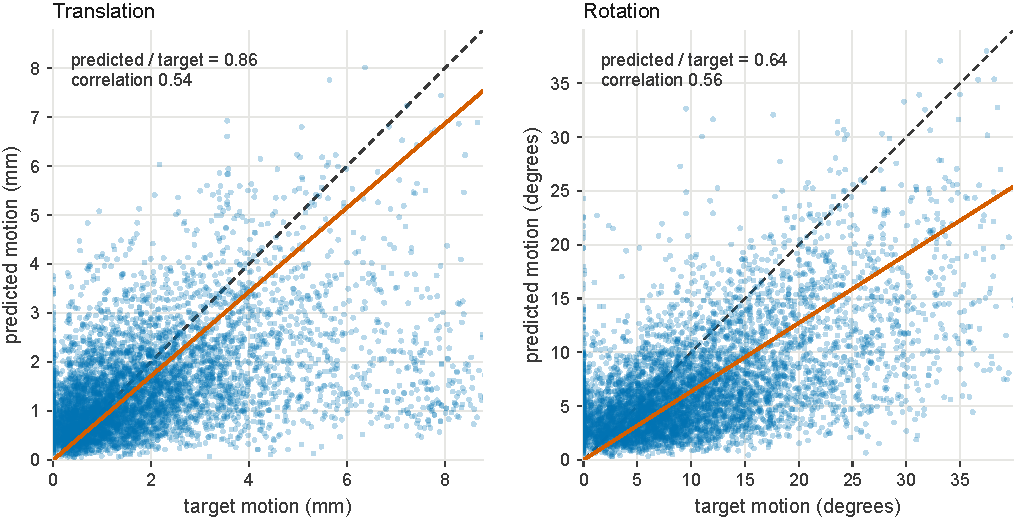
\includegraphics[width=\textwidth]{fig/calibration.pdf}
\caption{Predicted motion against the motion encoded by the simulated target transforms, with one point per tooth of the 246 test cases. The median predicted translation is 0.86 times the median target translation, with a correlation of 0.54, and the median predicted rotation is 0.64 times the median target rotation, with a correlation of 0.56. The dashed line denotes perfect calibration and the solid line the ratio of the medians.}
\label{fig:calibration}
\end{figure}

Figure~\ref{fig:case} shows the test case with the median point-cloud error of the fine-tuned model.

\begin{figure}[H]
\centering
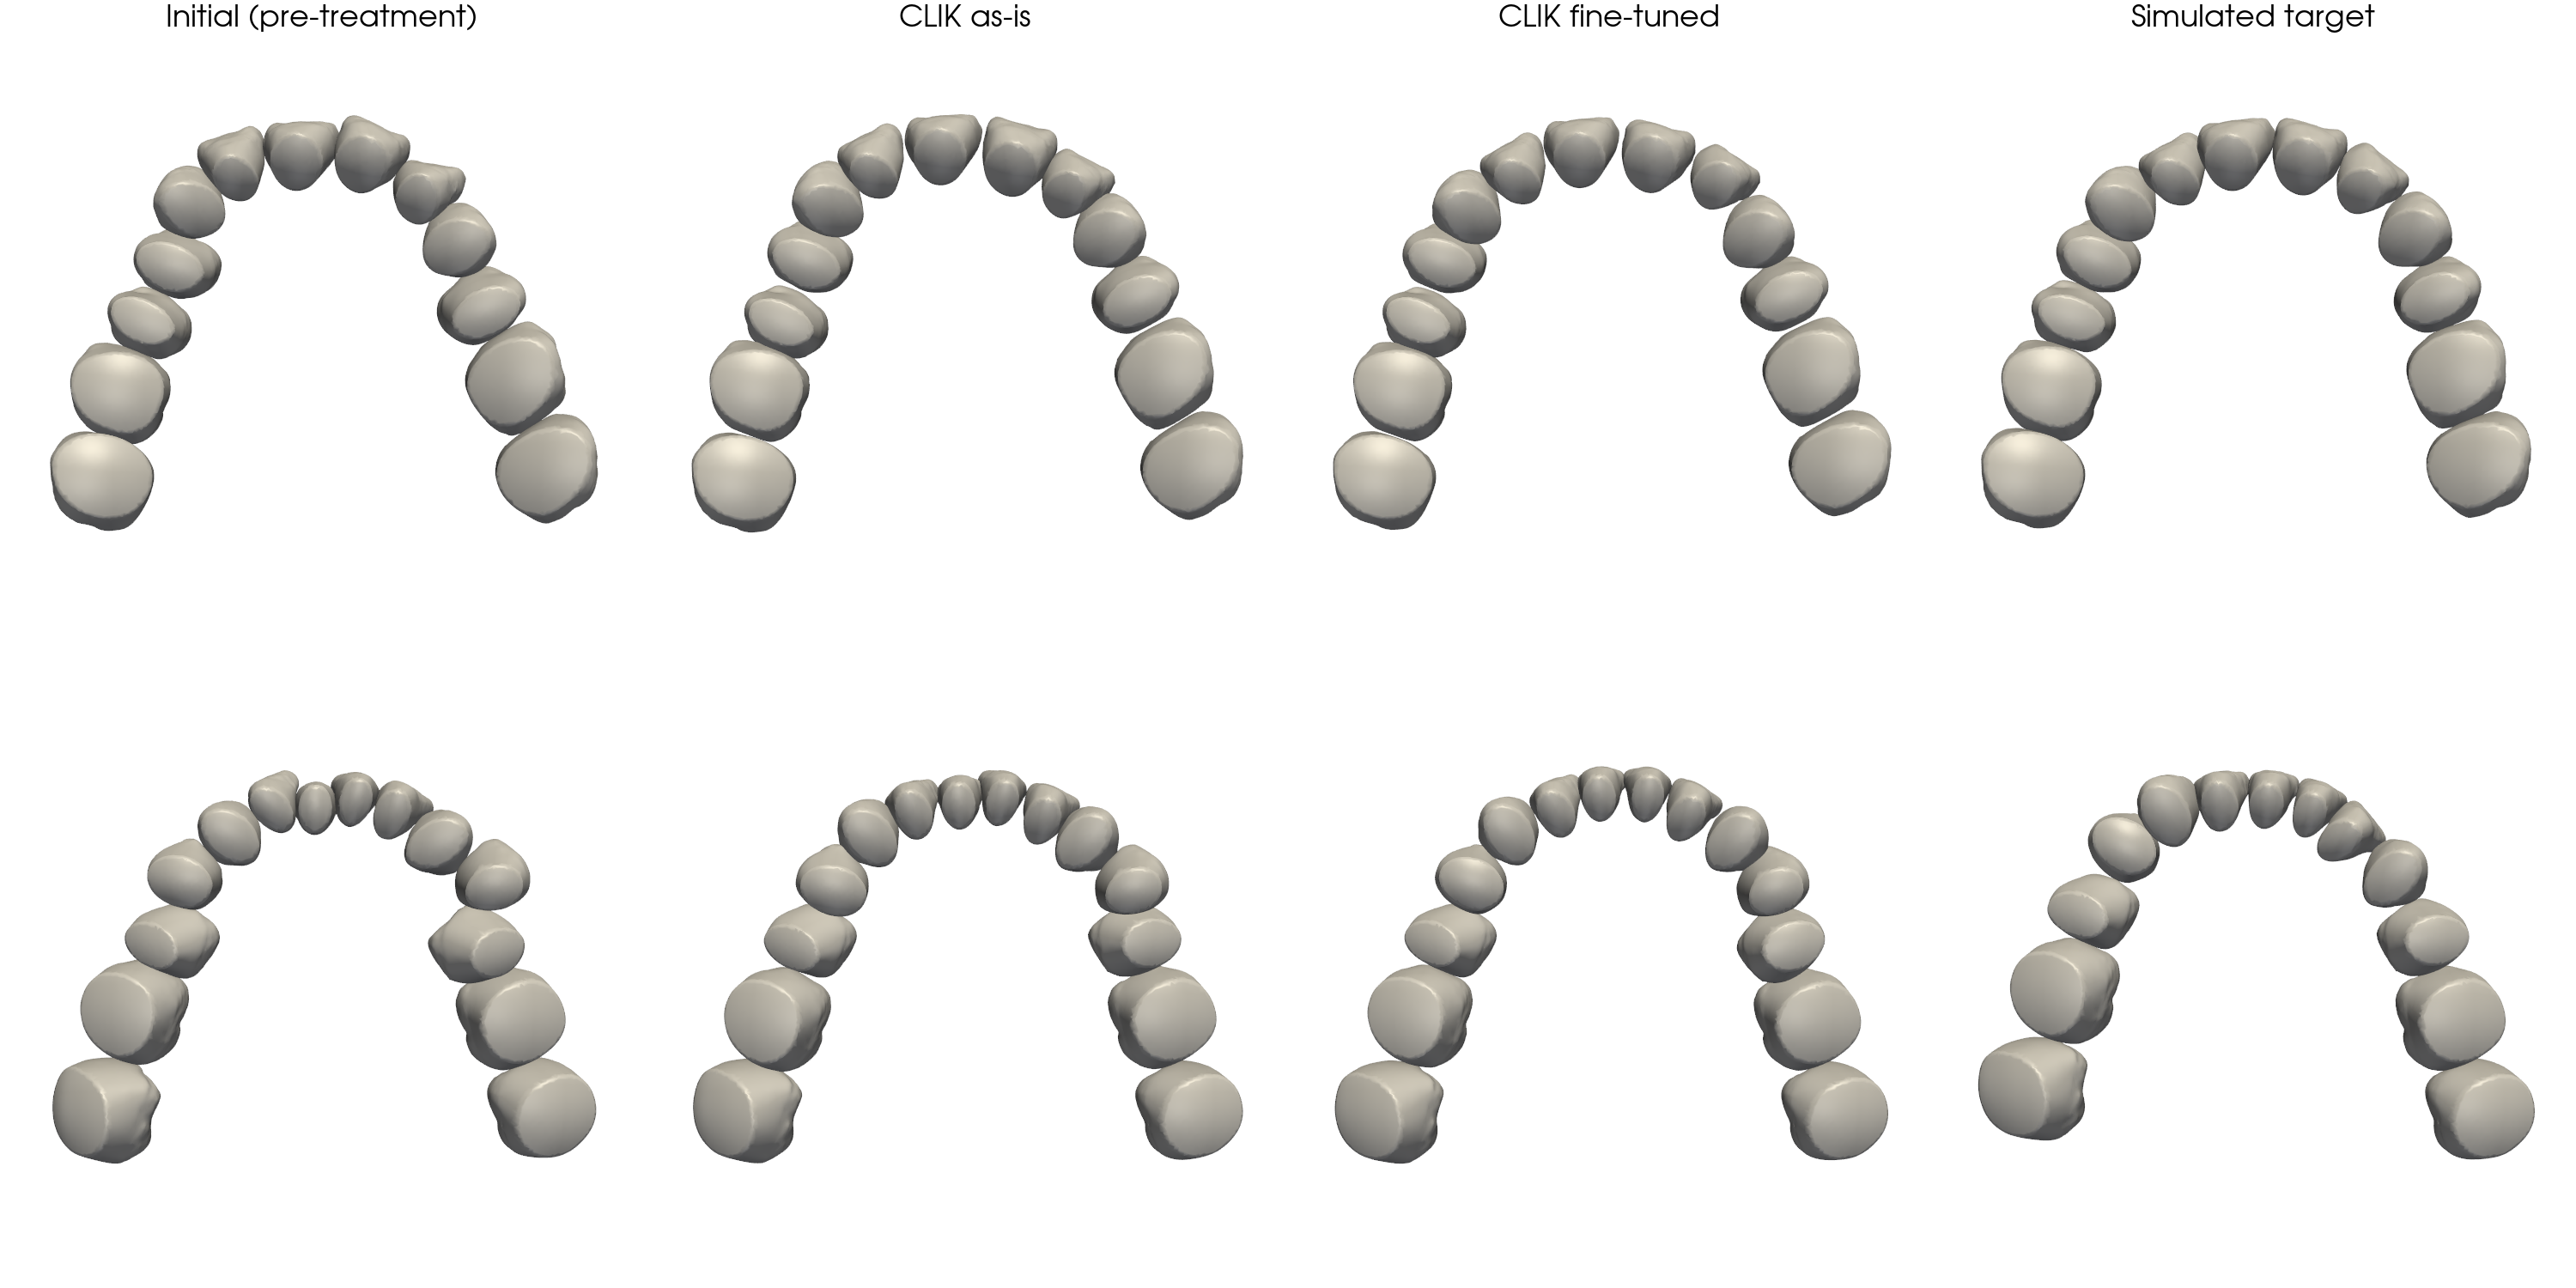
\includegraphics[width=\textwidth]{fig/0542_comparison.png}
\caption{The test case with the median point-cloud error of the fine-tuned model, with the upper arch above and the lower arch below, each seen from its biting surface: the pretreatment dentition, the predictions of CLIK as-is and of the fine-tuned model, and the simulated target.}
\label{fig:case}
\end{figure}

The two variants that check the training procedure changed little. Drawing the noise level from a continuous range, with everything else unchanged and both models evaluated on all 246 test cases with two hundred steps, gives 7.58\degree{} against 7.40\degree{} for the corresponding 100-epoch model, a significant deterioration of 2.4\% with $p = 0.002$. This shows that the continuous-noise variant performed worse under these settings; it does not establish whether the reconstructed discrete-noise procedure is correct. Tripling the number of epochs from 100 to 300 improves translation calibration, measured as the ratio between predicted and target motion, from 0.83 to 0.86, while the rotation ratio remains 0.64 and both correlations change by about 0.01. These results suggest a plateau well before 300 epochs.

Collision is measured on the first 40 test cases, with all four dentitions evaluated on the same cases, as shown in Table~\ref{tab:collision}. Fine-tuning reduces the median penetration depth from 0.397\,mm to 0.325\,mm and the share of penetrating points from 4.26\% to 3.24\%, but both remain well above the simulated target values of 0.141\,mm and 1.00\%, respectively. The collision term was omitted during this work's fine-tuning, so that adaptation did not directly penalize overlap. This does not mean that collision was absent from all training, since the published weights were trained using the original objective.

\begin{table}[H]
\centering
\small
\begin{tabularx}{\textwidth}{@{}Xrr@{}}
\toprule
Dentition & Median penetration & Penetrating points \\
\midrule
Before treatment  & 0.003\,mm & 0.24\% \\
CLIK as-is        & 0.397\,mm & 4.26\% \\
CLIK fine-tuned   & 0.325\,mm & 3.24\% \\
Simulated target  & 0.141\,mm & 1.00\% \\
\bottomrule
\end{tabularx}
\caption{Collision on the first 40 test cases, with all four dentitions evaluated on the same cases. The penetration depth of every dentition is the mean over its penetrating points, and the table gives its median over the cases together with the mean share of penetrating points. The surface points are sampled at random, and repeating the measurement with different points changes the depths by up to about 0.02\,mm.}
\label{tab:collision}
\end{table}




\subsection{Insensitivity to the noisy input and single-step sampling}
\label{sec:invariance}

The sensitivity measurement shows that the network does not use its noisy input. When eight clearly different noisy inputs are given at the same noise level, with the conditioning and everything else unchanged, the prediction changes by only four ten-thousandths of the variation of the input. This ratio is not only small but also nearly constant, between $4.2$ and $4.5\cdot10^{-4}$ at every level tested, from step 1999, where the input is almost pure noise, down to step 1. At high noise a small ratio is expected, because there the input carries little information and a good prediction of the clean landmarks has to rely on the conditioning. At step 1, instead, the input differs from the clean target by only about a tenth of a millimeter, so a network that used it would show a ratio close to one, whereas the measured ratio of $4.5\cdot10^{-4}$ means that even there the prediction is determined by the conditioning alone.

A direct consequence is that the number of denoising steps has almost no influence on the result. With the same checkpoint in both cases, a single step gives 7.35\degree{}, 1.36 and 1.58\,mm against 7.40\degree{}, 1.36 and 1.57\,mm with two thousand steps for the fine-tuned model trained for 100 epochs, and 9.27\degree{}, 1.85 and 2.57\,mm against 9.28\degree{}, 1.84 and 2.56\,mm for the published weights. All the differences are below one percent, and for the fine-tuned model none of them is significant, while for the published weights the rotation is not significant and translation and point cloud are worse by 0.15 and 0.34\%, a difference that 246 paired cases are enough to detect but that is about a hundred times smaller than the effect of fine-tuning on the same metrics. The same holds for the final model, where a single step gives 7.36\degree{}, 1.33 and 1.57\,mm against 7.38\degree{}, 1.32 and 1.58\,mm with the two hundred steps used throughout, without any significant difference ($p$ = 0.42, 0.22 and 0.11), and against 7.35\degree{}, 1.33 and 1.57\,mm with the full two thousand. Against the full chain only the point-cloud error differs significantly ($p = 0.02$), by 0.03\%, the same kind of difference, detectable but negligible, found for the published weights. In practice, a single network evaluation and two thousand produce the same dentition.

This behaviour belongs to the published model and was not introduced by the fine-tuning, since the same measurement on the weights released by the authors gives between $2.2$ and $2.7\cdot10^{-4}$, again nearly constant across noise levels. The most plausible explanation is the choice of predicting the clean landmarks instead of the noise. A network trained in this way can produce a complete answer from the conditioning alone, whereas a network trained to predict the noise could not, because the noise can only be recovered from the noisy input. The noise schedule gives the network little reason to read that input anyway, because on the scale of the coordinates it works on, which are millimeters divided by 46, the standard deviation of the noise exceeds 10\,mm from step 139 onwards and keeps growing, while the surface of a tooth moves by a median of 1.53\,mm in this test set, so that in more than 93\% of the training steps the noisy input carries little information about the motion beyond what the conditioning already provides. This explanation was not tested, since that would require retraining the model with the other target, and it is proposed as an interpretation of the results rather than as a finding. Its practical consequence is that the model behaves as a deterministic regression network, which maps every initial dentition to a single treated one, and loses the main advantage of a diffusion formulation, because an output that does not depend on the starting noise cannot provide alternative treatment plans, and the two thousand steps add nothing to a single prediction.




\section{Discussion}

The results include one expected finding and two unexpected ones, namely that the network ignores its noisy input and that it underestimates the size of the motion. That fine-tuning improves the model is not surprising, but it is informative that retraining only the diffusion stage, with the landmark detector left unchanged, is enough to reduce the point-cloud error from 2.56\,mm to 1.58\,mm. This does not establish that the detector identifies anatomically corresponding landmarks, which the class-by-class completion experiment supports only for some classes. One reading is that the published model failed on these cases because the treatment plans it learned differ from the simulated plans of this dataset rather than because of the landmarks, but this comparison does not isolate that mechanism.

The fine-tuned model underestimates the target motion, especially in rotation, although its predictions are positively correlated with it. One possible explanation is regression toward a conditional mean under squared-error training, since if similar inputs are paired with varied targets the prediction that minimizes the squared error is their average, which has a smaller magnitude than the individual motions. The present experiments do not test this mechanism, and since each case provides a single simulated target, the role of target ambiguity remains a hypothesis. The comparison with the mean-motion reference adds that in position the predictions are not yet more informative than the average motion of each tooth position, even though they clearly are in rotation and translation.


The measured insensitivity to the noisy input fits this hypothesis, because a network that ignores that input is a fixed function of the conditioning and would tend towards the conditional mean, and so does the rotation ratio that stays at 0.64 after 300 epochs, but neither observation proves that the loss is the limiting factor, and other causes may contribute.

The failure of the arch term may have a more specific cause. The term compares the five coefficients of a fourth-order polynomial fitted through the tooth centers, and the coefficients of a polynomial of that order are very sensitive, so that a small displacement of a single tooth can change them considerably, and the term may end up pushing the teeth towards matching coefficients rather than towards a better arch. It could also be suspected that the term suffers from being computed at a randomly drawn diffusion step, on a dentition that is still mostly noise, but that is not the case here, because the term is computed on the clean landmarks predicted by the network, and since that prediction does not depend on the noisy input the term sees almost the same finished dentition at every step. Weighting the term according to the noise level would therefore amount to little more than lowering its weight, and the two experiments that remain are a much smaller weight, since at 0.001 the term is still as large as the reconstruction loss, and a comparison of the two curves at the positions of the teeth instead of through their coefficients.

Why the orientation term helps is not established by these experiments, because the logged training loss contains the term itself and a comparison of generalization gaps would need its reconstruction part to be recorded separately.


\subsection{Limitations}
\label{sec:limitations}

The results of this work are subject to some limitations. Eleven cases, about one per cent of the collection, were excluded, and they were not excluded at random. Two cases are absent from the copy of the dataset available for this work, four lack the teeth needed to estimate the jaw frame, and four have different vertex counts between every pretreatment tooth mesh and its simulated-target counterpart, leaving no recoverable point correspondences. In the remaining case, conversion yields no teeth in the simulated target. This non-random exclusion may bias evaluation toward more complete and cleanly acquired dentitions. The dataset, moreover, does not distribute patient identifiers, so different scans of the same patient may appear in both the training and the test data, which could make the test results optimistic, and only the reuse of identical scans could be checked, which affects four test cases without changing the results.

The ablation has a similar limitation: it was run on the first 100 test cases to keep the cost of six training runs manageable. These cases have lower no-movement-reference errors than the full 246-case test set (8.95\degree{}, 1.68 and 1.52\,mm, compared with 9.49\degree{}, 1.76 and 1.72\,mm, respectively). Since each variant is compared with the reconstruction-loss reference on the same cases, the comparisons are paired. However, this subset may not represent the full test set, and the absolute ablation values should not be compared directly with the full-test-set values.

The number of epochs is also much lower than in the original work, 300 against 10000, but the flat validation loss and the nearly unchanged results after tripling the epochs suggest that longer training would not change the conclusions.

Two further limitations concern the method rather than the computational budget. The first is the landmark representation, since some landmark indices do not correspond to a stable anatomical position across patients, and it is not possible to check whether the same happens on the data CLIK was trained on, because that data is not public. The second is that the collision term was never implemented, and the fine-tuned predictions still show more than twice the penetration depth and three times the share of penetrating points of the simulated targets.

All metrics measure geometric agreement with a single digitally simulated plan approved by an orthodontist, so they neither assess clinical quality nor account for alternative plans that would be equally valid, and whether the predictions are clinically acceptable could only be judged by an orthodontist.

These limitations also suggest how this work could continue. Implementing the collision term, possibly with a larger weight than the published one, would show whether the overlap that fine-tuning leaves well above the level of the simulated targets can be reduced, and a much smaller arch weight, together with a point-by-point comparison of the arch curves, would show whether the arch constraint can be made useful. Retraining the landmark detector together with the diffusion model would show whether the instability of the anterior landmarks can be reduced. Training the same network to predict the noise instead of the clean landmarks would test the explanation proposed for its insensitivity to the noisy input, while if a single prediction is all that is needed the diffusion formulation could be dropped in favor of a plain regression network with the same inputs, which is what the current model already is in practice. The most important change, however, would be to replace the squared error with a loss that does not converge towards the average of the plausible plans, which is what a diffusion model is supposed to avoid and would show whether that averaging contributes to the underestimated motions. Such a model would probably obtain worse scores on the metrics used here, because it would still be compared with a single simulated plan, and its advantage would be the ability to propose alternatives rather than a higher accuracy.


\section{Conclusion}

The landmark detector of CLIK transfers to intraoral scans as a detector of positions, since its landmarks lie at a median distance below a millimeter from the annotations of four of the six classes and the other two can be computed from the geometry of the crown, but its landmarks cannot be mapped reliably onto the annotated classes one by one.

Used as-is on intraoral scans, CLIK produces lower error than the no-movement reference in 44\% of the cases for rotation, 33\% for translation and 17\% for point-cloud distance. Fine-tuning only the diffusion stage, on 703 training cases for 300 epochs, brings all three median errors below that reference and raises these shares to 70\%, 69\% and 55\%, and the fine-tuned model also beats the average motion of each tooth position in rotation and translation, though not in position, where its advantage is not significant. These results measure geometric agreement with simulated targets and do not establish clinical benefit, which only orthodontists could judge.

Of the implemented constraints, tooth orientation improves the results, contact has no measurable effect, and the arch term is harmful at the weights tested, possibly because of its scale. Finally, the diffusion network ignores its noisy input, so that a single denoising step gives the same metrics as the full chain for the published weights and for the fine-tuned models, and the model behaves in practice as a deterministic regression network from the initial dentition to a single treated one.


\bibliographystyle{plainnat}
\bibliography{refs}

\end{document}
